\section{Platform}
\label{sec:platform}

We used the PR2 research robot from Willow Garage shown in Fig.
\ref{fig:PR2} for the 2015 APC competition. The robot consists of two
7-DOF manipulators attached to a height-adjustable torso and equipped with parallel-jaw
grippers. A pan-tilt controllable robot head is located on the upper part of the robot
and equipped with a set of RGB cameras and a Kinect camera which we used in
our object segmentation system. The robot is also
equipped with a tilt-controllable laser scanner located right beneath the head which we
also used for object segmentation purposes.
A set of 4 wheels at the base provides the robot with omnidirectional mobility, which we
exploited in order to control the robot back and forth from the shelf to pick up objects
and release them in the target box.


\begin{figure}[h]
\centering
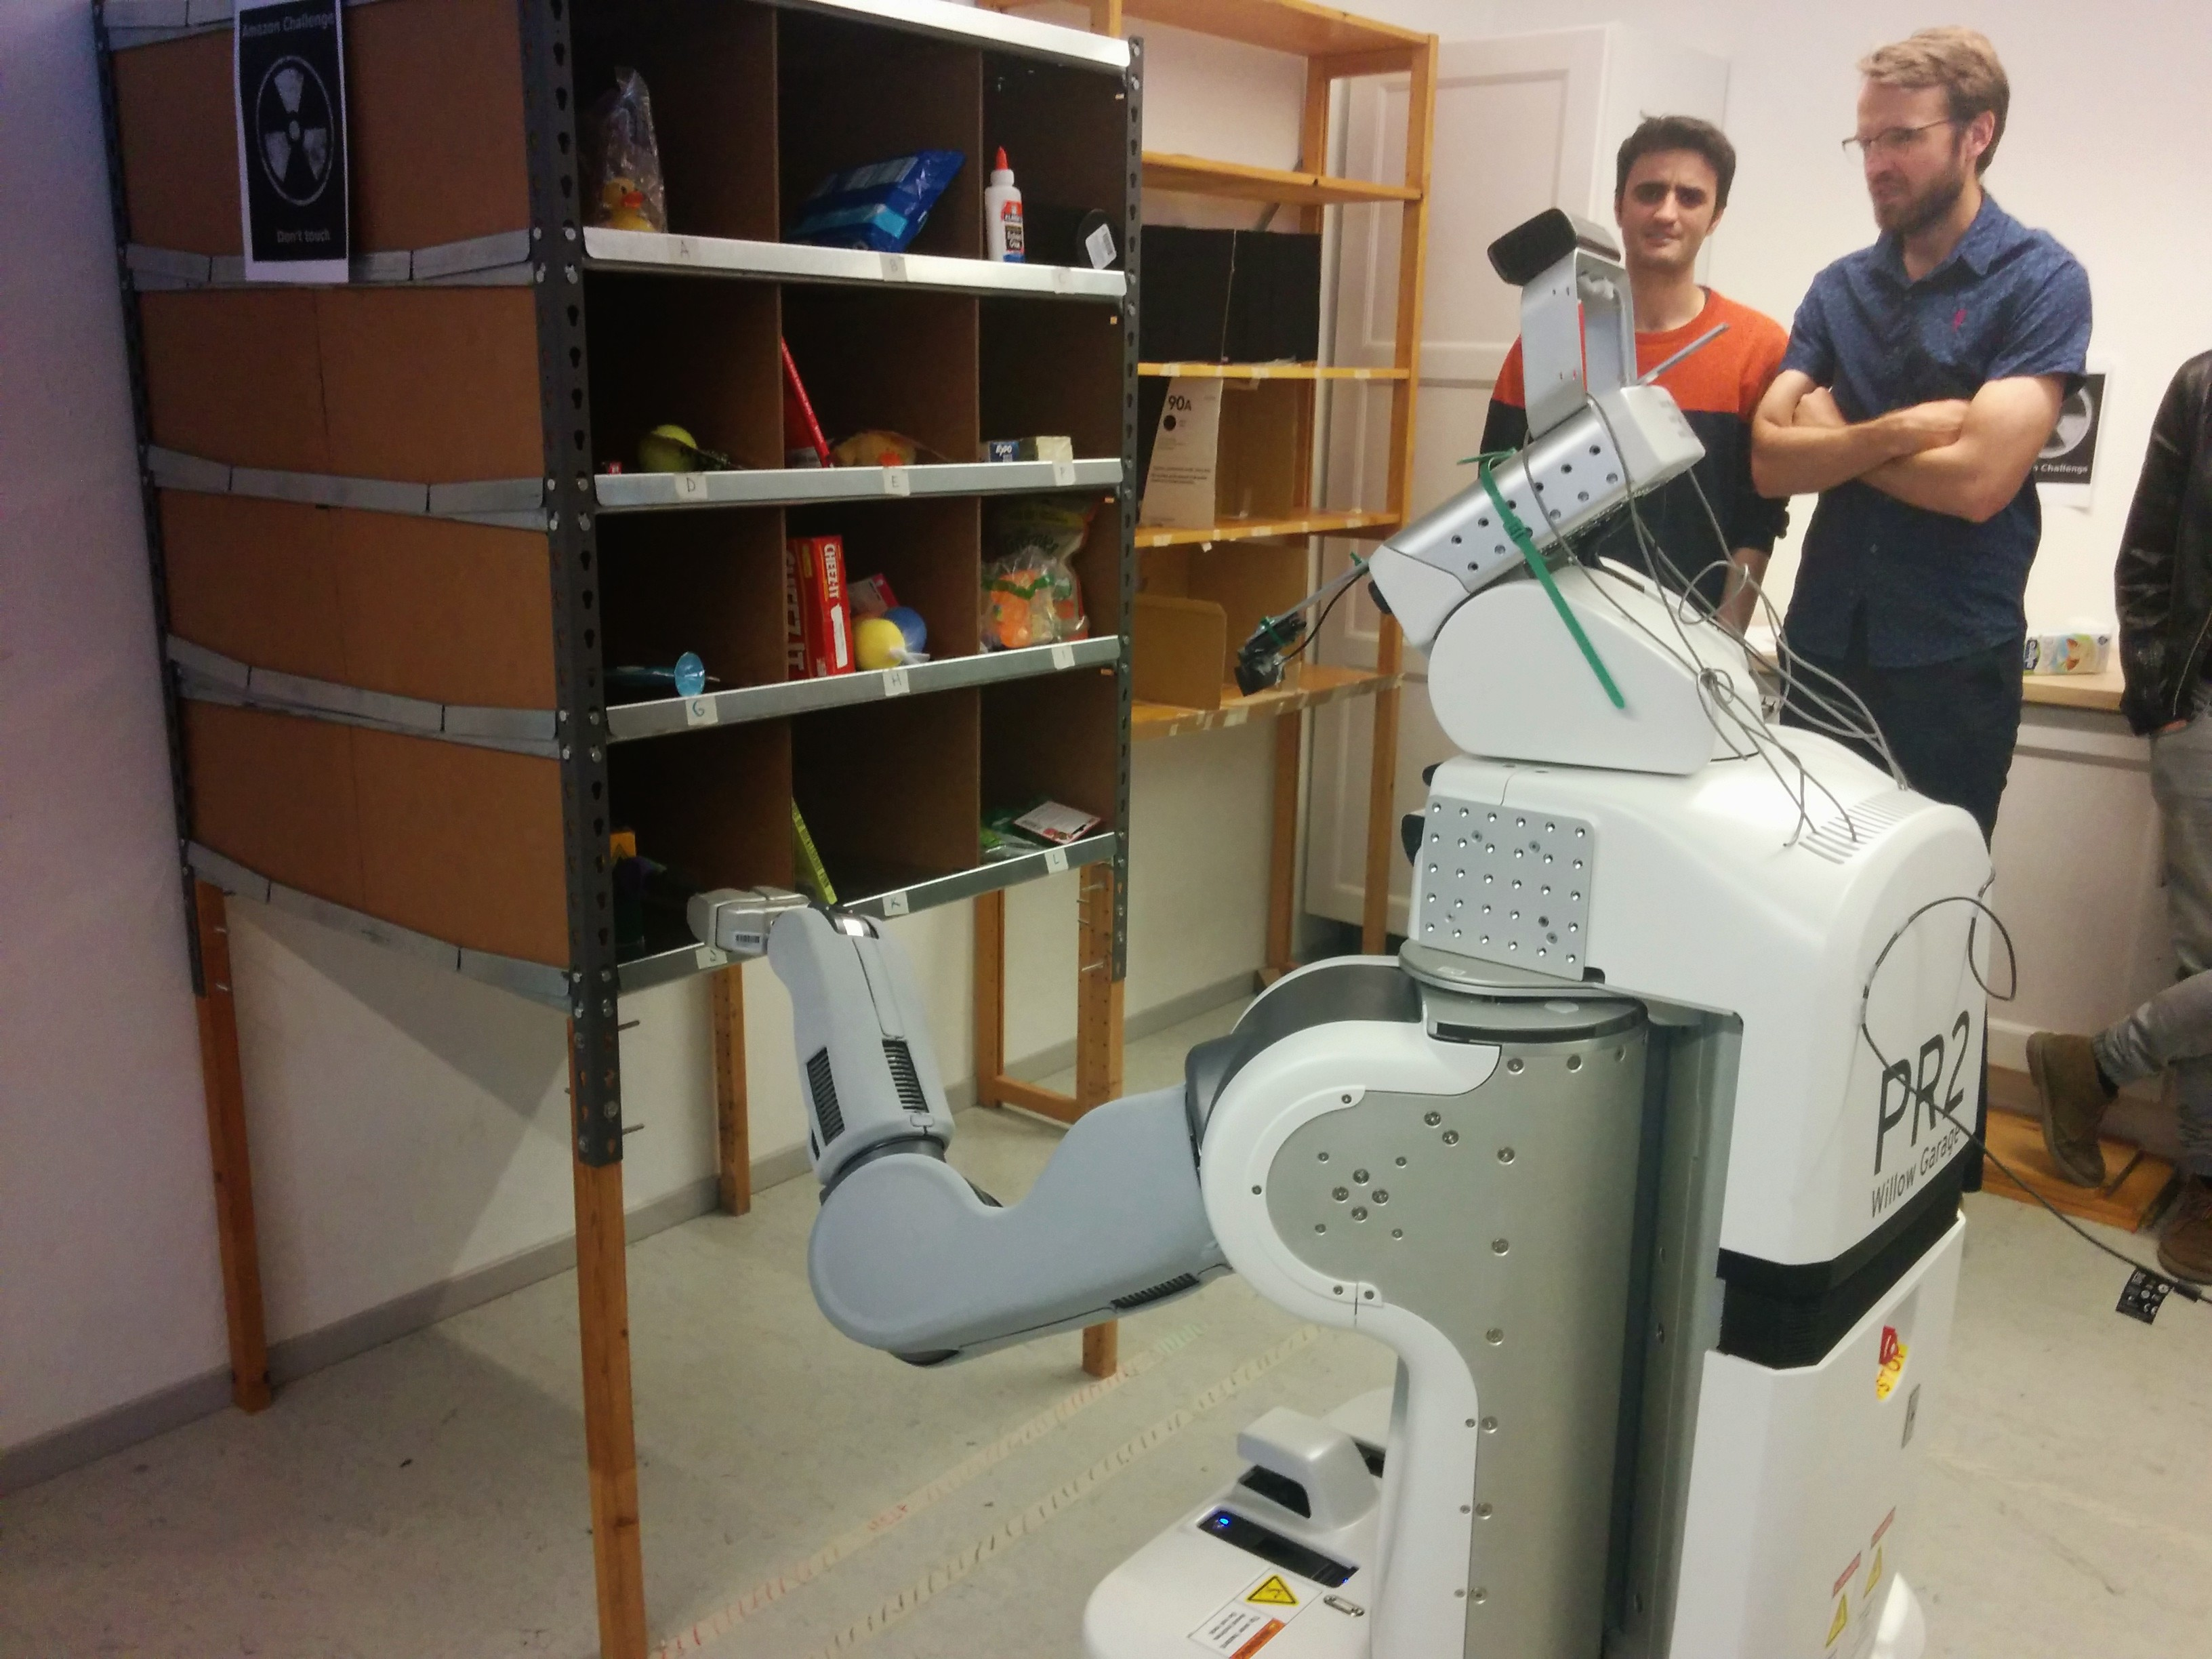
\includegraphics[trim=15.0cm 4.0cm 6.0cm 0cm,clip=true,scale=0.07]{figures/pr2.jpg}
\caption{Team CVAP's PR2 robot platform used for the Amazon Picking Challenge 2015 in Seattle, USA.}\label{fig:baxter}
\end{figure}

We provided some minor hardware modifications to the PR2 robot in order to
address some of the challenges  of the picking task,
namely custom-made extension fingers for the parallel gripper in order
to be able to reach further inside of the bins of the shelf and a high resolution
webcamera which we attached on the PR2's head in order to get
a richer set of image features for our Simtrack vision system to detect the target 
objets in the shelf.

The robot ran on an Ubuntu 12.04 computer with a real-time linux kernel that provides
1 KHz manipulator control. All the high level task execution, perception, grasping and manipulation software components were developed under the Robot Operating System (ROS).
